\section{Construction of icosahedral grid}
The icosahedral geodesic grid is constructed as follows:
\begin{enumerate}
  \item Each side of the icosahedron whose vertices are on a unit sphere are
    projected onto the sphere. This grid is called 'glevel 0' gri. (Fig. \ref{fig:scale-gm_grid}(a)).
  \item By connecting the mid-points of the geodesic arcs, four
      sub-trianbles are generated from each of the 'glevel 0' triangles. This
      grid is called 'glevel 1' grid (Fig. \ref{fig:scale-gm_grid}(b)).
  \item By iterating this process $l$-th times, a grid structure of 'glevel l'
    is obtained. 
\end{enumerate}
The total number $N_p$ of triangle verrtices with the glevel $l$ grid can be
described as 
\begin{equation}
  N_p(l) = 10 \times 4^l + 2 \nonumber
\end{equation}

\begin{figure}[H]
  \begin{center}
    \includegraphics[width=10cm]{../../figure/grid_structures}
%    \begin{tabular}{cc}
%    \includegraphics[width=5cm]{../../figure/grid0} &
%    \includegraphics[width=5cm]{../../figure/grid1} \\
%    \includegraphics[width=5cm]{../../figure/grid2} &
%    \includegraphics[width=5cm]{../../figure/grid3}
%    \end{tabular}
    \caption{Grid structure (grid division levels 0-3).}
    \label{fig:scale-gm_grid}
  \end{center}
\end{figure}


\section{Control volume}
All the  variables are defined at the vertices of triangles. This arrangement
is so-called 'Arakawa-A' type grid. Since the descritization of equations is
based on the finite volume method, it is necessary for the control volume to
be defined. The schematic figure of control volume is shown in Fig. \ref{fig:scale-gm_control_volume}. The
red points of $P_0$ up to $P_6$ are the vertices of triangles, Green points
remained are defined as gravitational center of the corresponding
triangles. The control volume for the point $P_0$ is defined as the polygon
constructed by connecting the gravitational centers of the neighbouring
triangles. The shape of control volume in the almost region is hexagon, while
it is pentagon at only 12 points inherited from glevel 0.

\begin{figure}[H]
  \begin{center}
    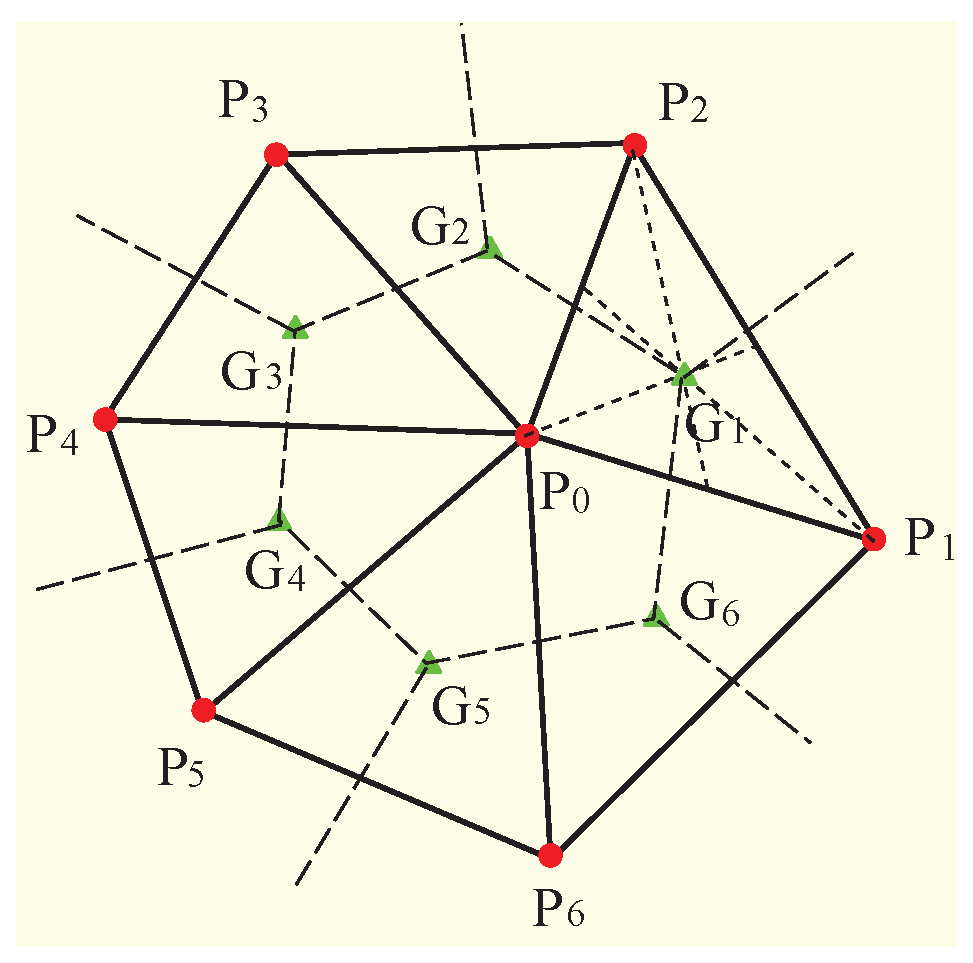
\includegraphics[width=5cm]{../../figure/control_volume}
    \caption{Schematic figure of the control volume}
    \label{fig:scale-gm_control_volume}
  \end{center}
\end{figure}


\section{Modification of icosahedral grid}
The construction method of control volume as described in the previous
subsection has one problem as regards to accuracy. From the viewpoints of
accuracy, any variable-defined point should be the gravitational center of
control volume. However, it is not so in the above construction. So, we
develop a new grid by modifying the default grid as follows.
\begin{enumerate}
  \item After the construction of first control volume by the previous method,
    variable-defined points are moved to the gravitaitonal center of control
    volume. This process is shown in Fig. \ref{fig:scale-gm_modified_control_volume}. The blue points are new
    locations of variable-defined points.
  \item By using the new location of variable-defined points, next
    variable-defined points are obtained in the same manner.
  \item This iteration is reported until the variable-defined points is
    converged.
\end{enumerate}
Whether grid is converged or not has not been yet mathematically proved, but
practically, it can be converged up to glevel 8. Those grids are called glevel
$l$M.

\begin{figure}[H]
  \begin{center}
    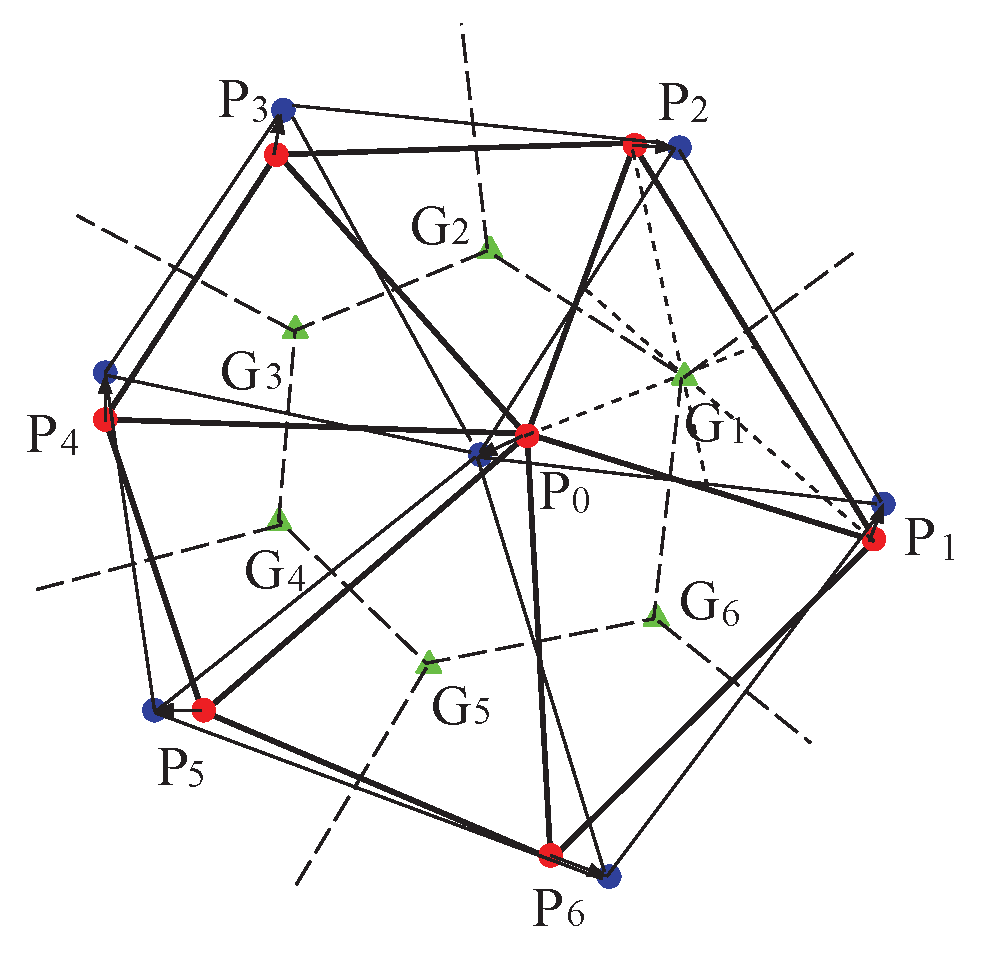
\includegraphics[width=5cm]{../../figure/modified_control_volume}
    \caption{Schematic figure of modified grid and control volume}
    \label{fig:scale-gm_modified_control_volume}
  \end{center}
\end{figure}


Figure \ref{fig:scale-gm_control_volume_comparison} gives the default grid and modified one for the grid division level
3. As shown in this figure, the grid interval around vertices of icosahedron
slightly decreases by the modification. This lead to the increase of
maximum/minimum ratio of grid interval. 
%The maximum/minimum ratio of grid
%interval against grid division level is shown in Fgi. XX, where grid interval
%$d$ is defined as the root of control volume area. It can be guessed from this
%figure that even in the glevel 11M grid the value of $d_max/d_min$ will be
%about 3, so it is enough acceptable. 

\begin{figure}[H]
  \begin{center}
    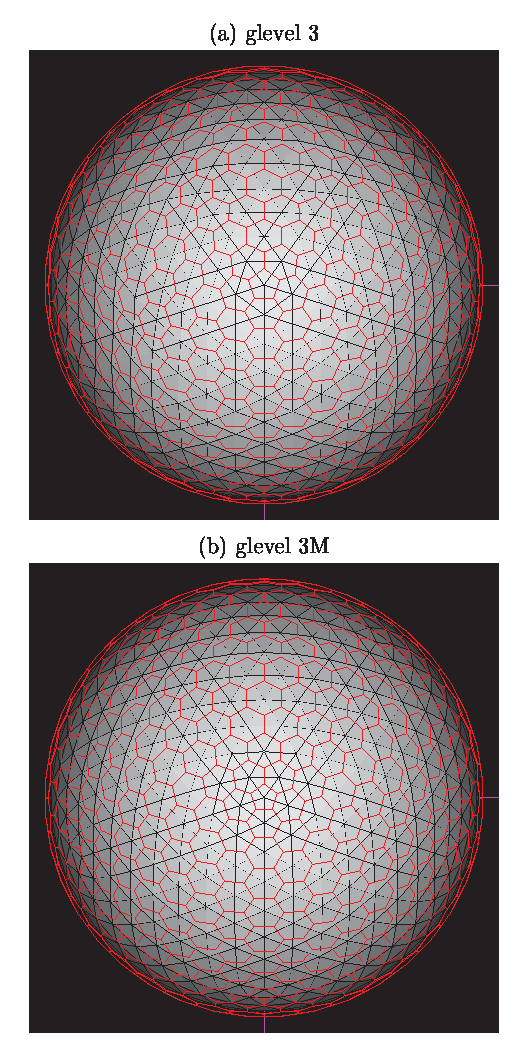
\includegraphics[width=5cm]{../../figure/control_volume_comparison}
    \caption{Comparison of default and modiified grids. The perspective
      center of the figures is located at the north pole.}
    \label{fig:scale-gm_control_volume_comparison}
  \end{center}
\end{figure}



\section{Parallelization}
\subsection{Region division}
The concept of region division level is introduced as follows.
\begin{enumerate}
  \item By connecting two neighboring triangles of spherical icosahedron, ten
    rectangles are constructed as Fig. \ref{fig:scale-gm_region_structure}(a). This construction is called 'rlevel
    0.'
  \item For each rectangle, four sub-rectangles are generated by connecting
    the diagonal mid-grid-points (Fig. \ref{fig:scale-gm_region_structure}(b)). This construction is called
    'rlevel 1.'
  \item This process is repeated until the desirable regions are obtained.
\end{enumerate}
This example of grid structure in a region is shown in Fig. \ref{fig:scale-gm_grid_structure}. Although the
grid is not based on rectangles but triangles, it is like a
structured-grid. On the other words, all variables can be described by
Fortran's 2 dimensional array. This is an advantage for vector super-computing.

\begin{figure}[H]
  \begin{center}
    \includegraphics[width=10cm]{../../figure/region_structure}
    \caption{Region structure (region division levels 0-3)}
    \label{fig:scale-gm_region_structure}
  \end{center}
\end{figure}

\begin{figure}[H]
  \begin{center}
    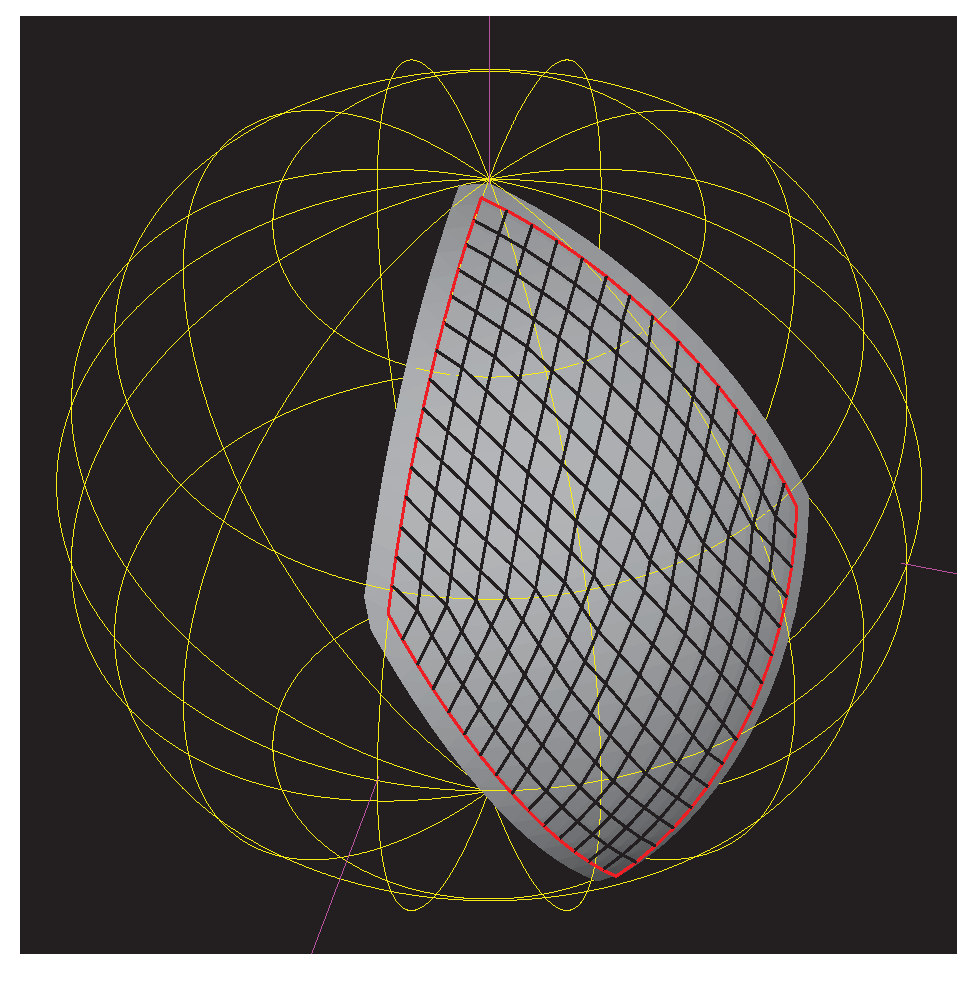
\includegraphics[width=5cm]{../../figure/grid_structure}
    \caption{Grid structure of one region.}
    \label{fig:scale-gm_grid_structure}
  \end{center}
\end{figure}


\subsection{Parallelization}
In the parallel computing, the regions made by the above method are managed by
some processes. One of the simples solutions of parallilization is that one
process manages one region. However, it is lacking of flexibility. We design
the management of region as follows.
\begin{enumerate}
  \item Any process can manage any nubmer and any location of regions.
  \item Number of managed process is not necessary to be constant.
\end{enumerate}
This design concept makes the load of each CPU be uniform.

When two neigouring regions are not managed by the same process, the excahnge
of boundary conditions is done using MPI communication. When two neighboring
regions are managed by the same process, it is done by copying the memory of
boundary.

Figure \ref{fig:scale-gm_parallel} shows the schematic figure of region management. This figure is an
expansion for rlevel 1. Total amount of region is forty and ten processes
manage those regions. Each of the processes manages the region marked by same
color. For example, regions A, B, C, and D are managed by the same process. It
is configured for each fo processes to manage the regions from pole and
equatorial regions. By this configuration, locad imbalance due to the
atmospheric physical process would be avoided.

\begin{figure}[H]
  \begin{center}
    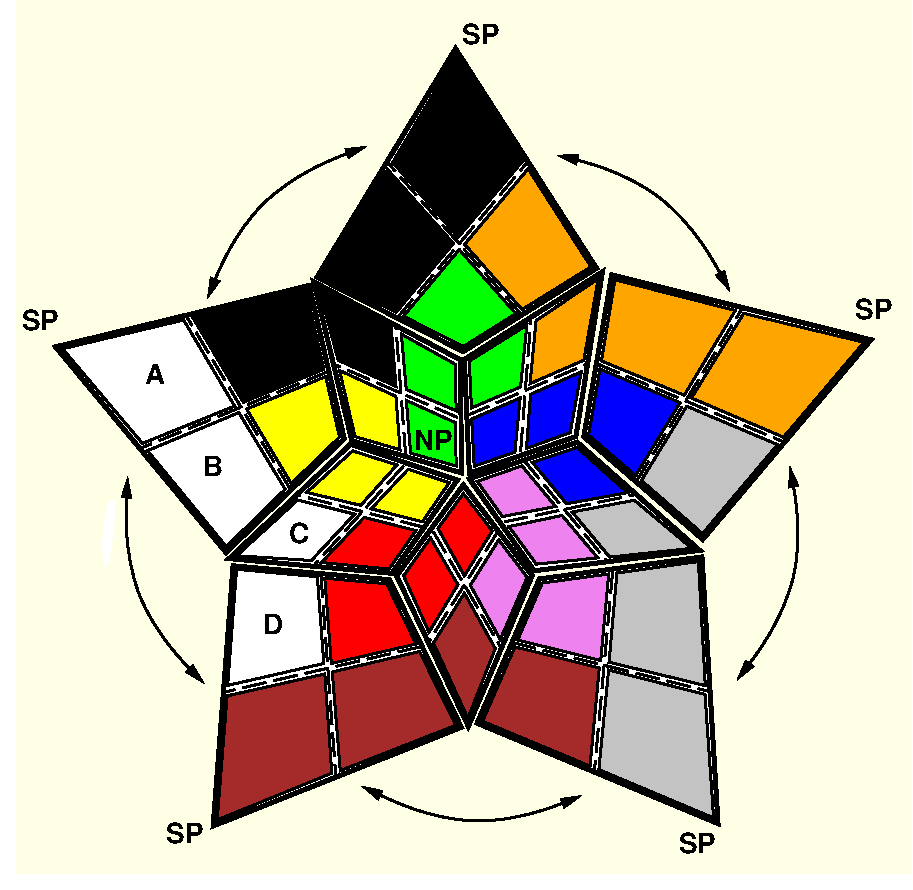
\includegraphics[width=5cm]{../../figure/parallel}
    \caption{Schematic figure of parallelization.}
    \label{fig:scale-gm_parallel}
  \end{center}
\end{figure}



\subsection{Note}
 \begin{itemize}
   \item g-level (grid level): number of subdivision times of the grid from the original icosahedron.
         the number starts from 1, we recommend to use the number larger than 4.
   \item r-level (region level): number of subdivision times of the region(tile)
         from the original icosahedron. When r-level = 0, we have ten regions(tiles).
         At that time, the number of available maximum MPI processes is ten.
 \end{itemize}

\textcolor{red}{[さらにHALOを説明する図もある方が良い]}

